\item Dos tubos de altura H, diámetro interno $d_i$ se encuentran conectados a un tanque pequeño. Los tubos y el tanque contienen agua. El sistema se encuentra unido a una plataforma, como se muestra en la figura \ref{fig:tuboU}. A qué velocidad angular $\omega$ debe girar la plataforma, de manera que la configuración de estado permanente del agua haga que ésta alcance la parte superior del tubo exterior? No tenga en cuenta los efectos de capilaridad. Exprese la solución en términos de las siquientes variables:

%% Esto son datos centrados
\begin{center}
%$\H = 16 \{cm} \d_i = 0,2 \{cm} $\\
%$\D = 8 \{cm} \h = 10 \{cm}$
$H \qquad d_i \qquad D \qquad \Delta h \qquad r$
\end{center}

%% Esto es una figura
\begin{figure}[h!!!!]
\centering
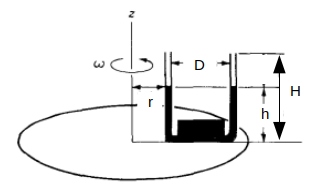
\includegraphics[width=0.5\textwidth]{tuboU.png}
\caption{Tubo en U descentrado}
\label{fig:tuboU}
\end{figure}
